\section{Overview: Results of Dataset}
\section{Discussion}
\subsection{Comparision to Experiment}

\begin{figure}
	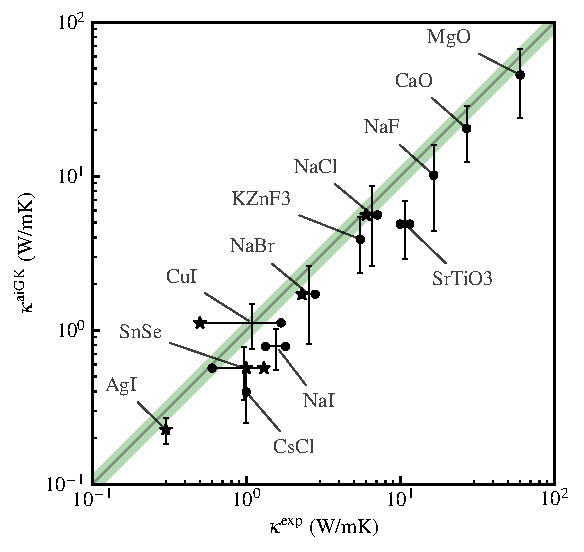
\includegraphics[width=\textwidth]{./data/plots/kappa_vs_exp/kappa_vs_exp.pdf}
	\caption{Comparison to experiment. Bullets($\bullet$): Single crystal. Stars ($\star$): Polycrystalline or thin-film experiment. Error bar in y-directioin: Statistical uncertainty for $\kappa^{\rm aiGK}$ from standard error over individual trajectories and Cartesian components~[ref]. Green band: Agreement between mean experiment and mean computation with $\pm 15\,\%$ deviation.}
	\label{fig:kappa_exp}
\end{figure}

\subsection{Relation to Anharmonicity}

\begin{figure}
	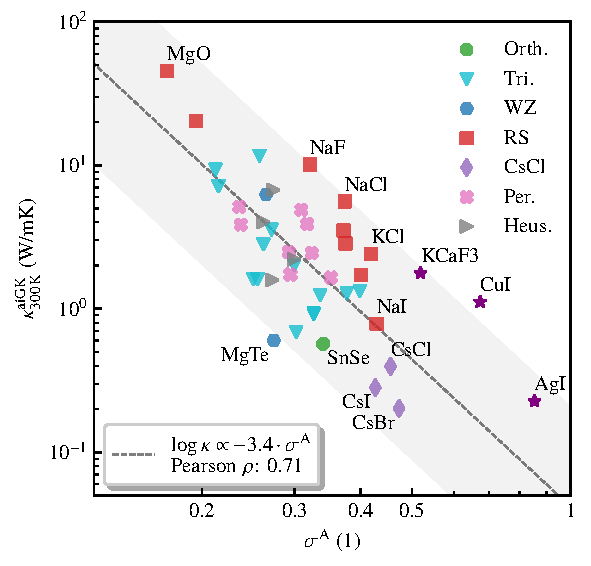
\includegraphics[width=\textwidth]{./data/plots/kappa_vs_sigma/kappa_vs_sigma.pdf}
	\caption{Thermal conductivity at room temperature vs. anharmonicity measure.}
	\label{fig:kappa_sigma}
\end{figure}

\section{Dynamical Effects}

\subsection{CuI}

\begin{figure}
	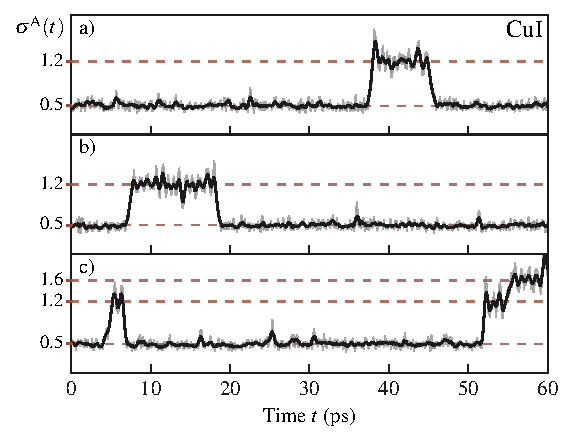
\includegraphics[width=\textwidth]{./data/plots/defects/216.02.CuI/sigma_vs_time.pdf}
	\caption{Zincblende (SG\,216) CuI, describe}
	\label{}
\end{figure}

\begin{figure*}
	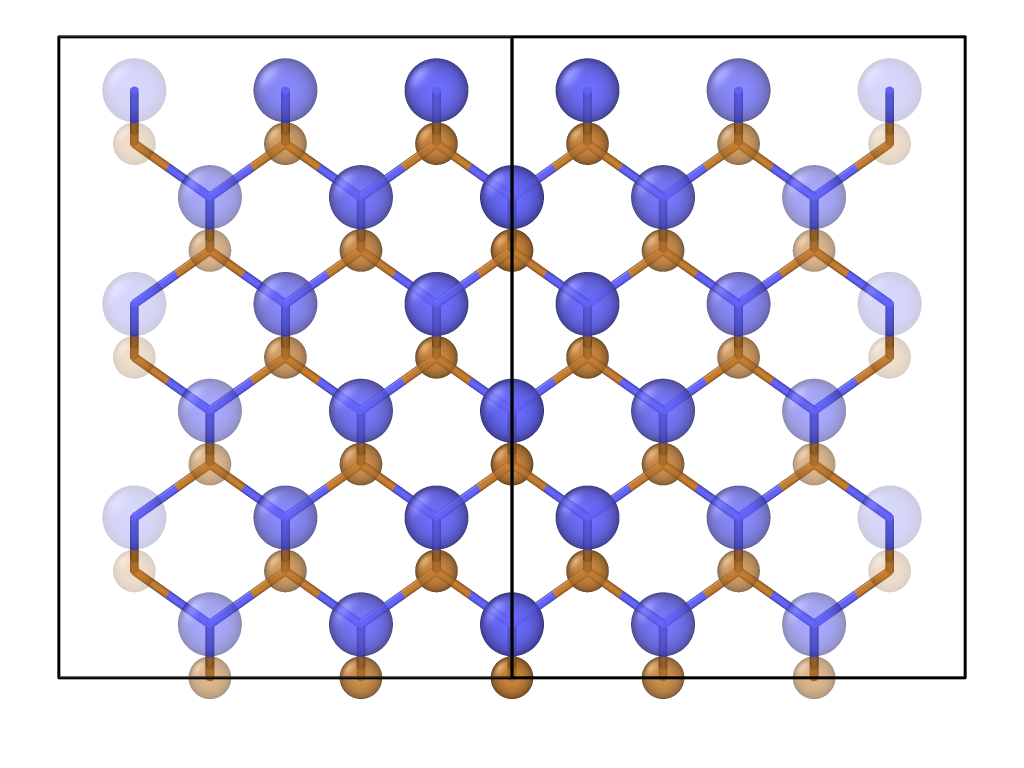
\includegraphics[width=.5\textwidth]{./data/plots/defects/216.02.CuI/perfect_110_solid.png} \hfill
	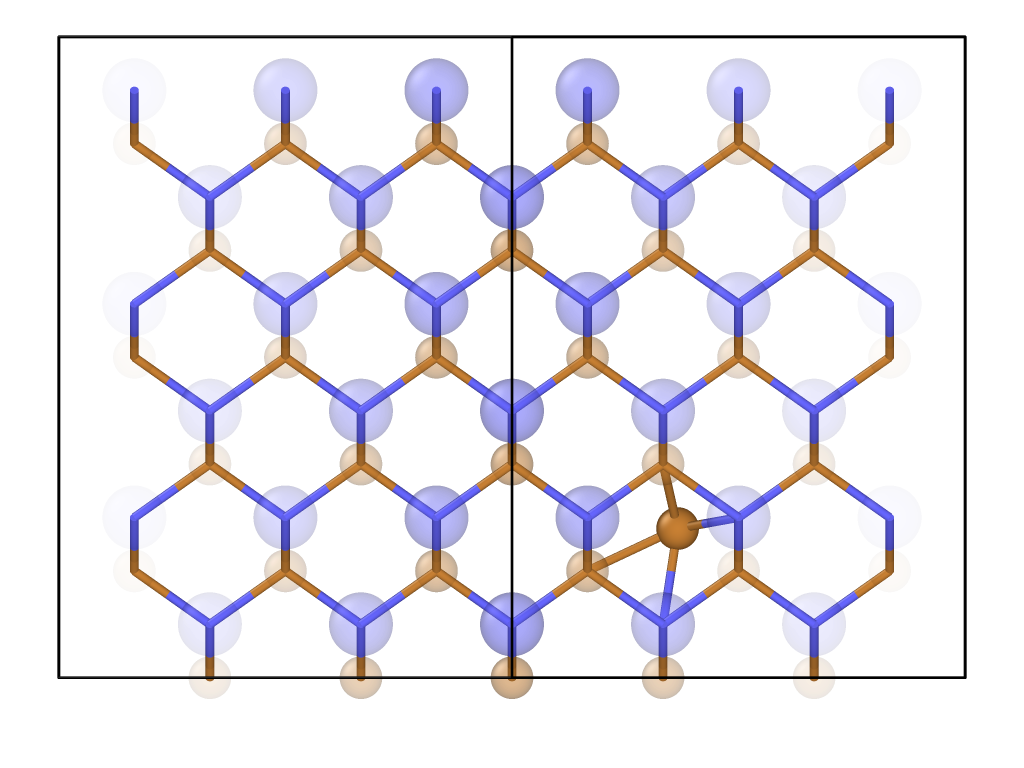
\includegraphics[width=.5\textwidth]{./data/plots/defects/216.02.CuI/defect_110.png}
	\caption{CuI viewed in (110) direction. Left: High-symmetry zincblende structure. Right: Copper ion in lower-right quadrant moves into interstitial site along (111) direction.}
	\label{}
\end{figure*}

\begin{figure*}
	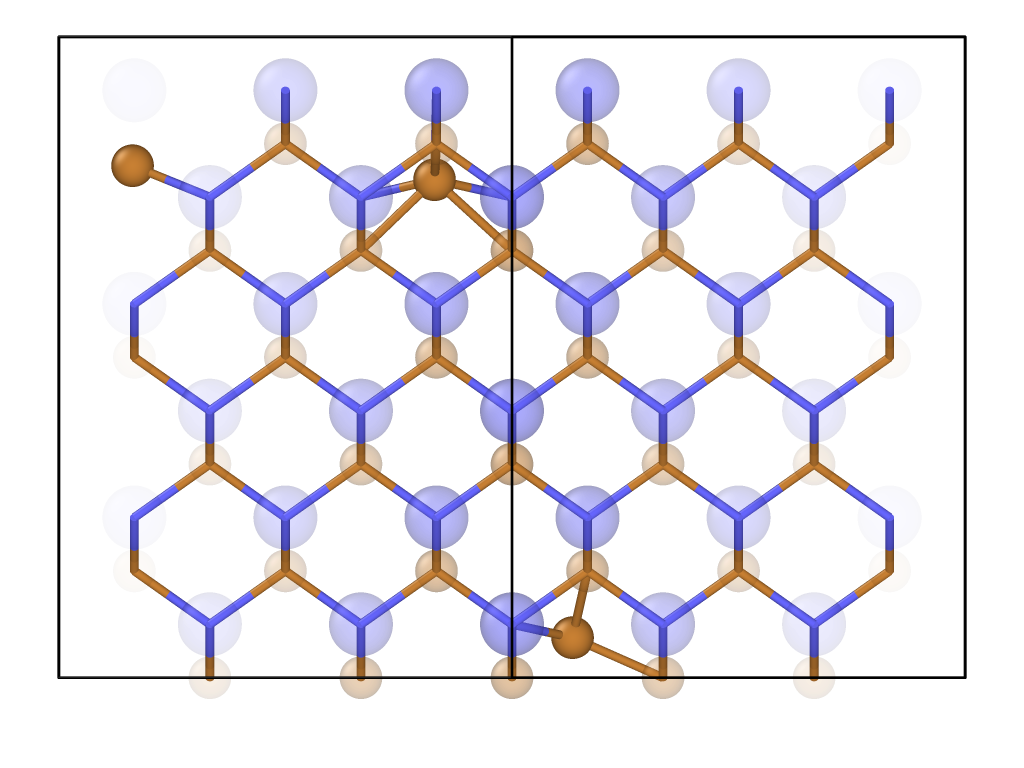
\includegraphics[width=.5\textwidth]{./data/plots/defects/216.02.CuI/defects_110.png} \hfill
	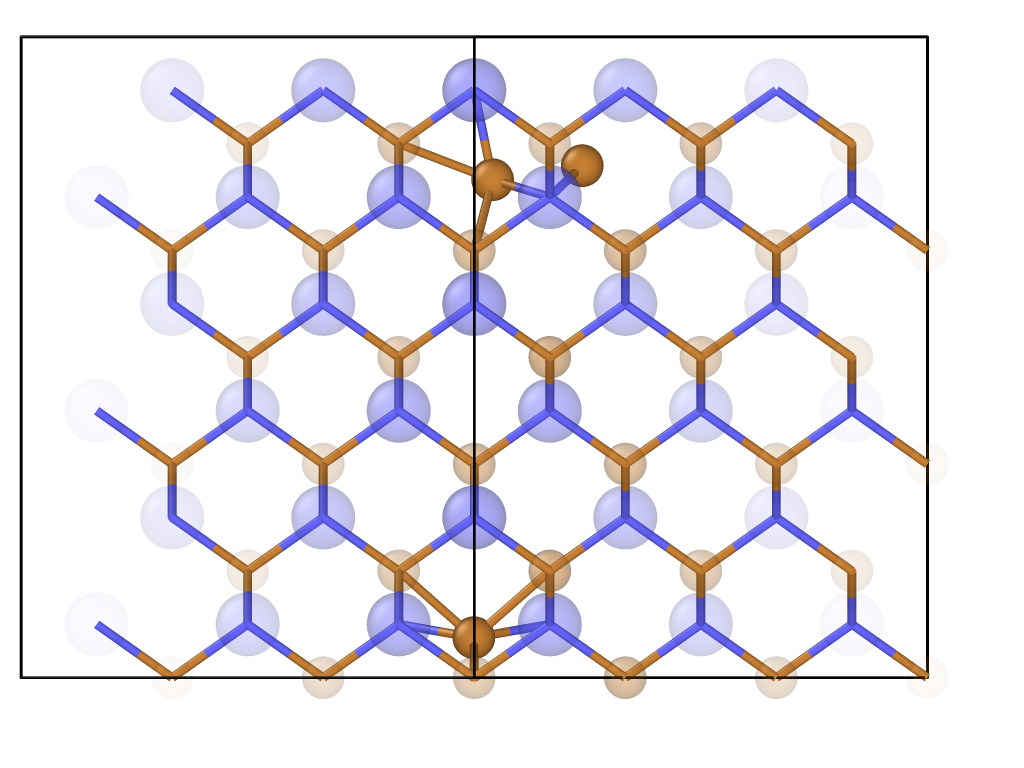
\includegraphics[width=.5\textwidth]{./data/plots/defects/216.02.CuI/defects_110_135.png}
	\caption{2.5 defects in (110) and rotated by 90\,deg about z-axis.}
	\label{}
\end{figure*}

\subsection{KCaF$_3$}

\begin{figure}
	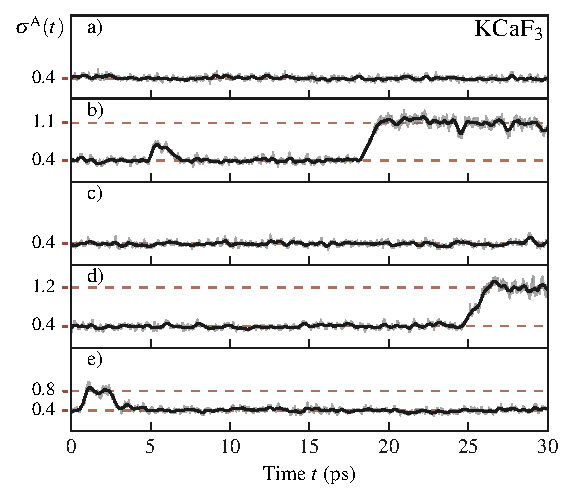
\includegraphics[width=\textwidth]{./data/plots/defects/062.05.KCaF3/sigma_vs_time.pdf}
	\caption{Orthorombic (SG\,62) KCaF$_3$, describe}
	\label{}
\end{figure}

\begin{figure*}
	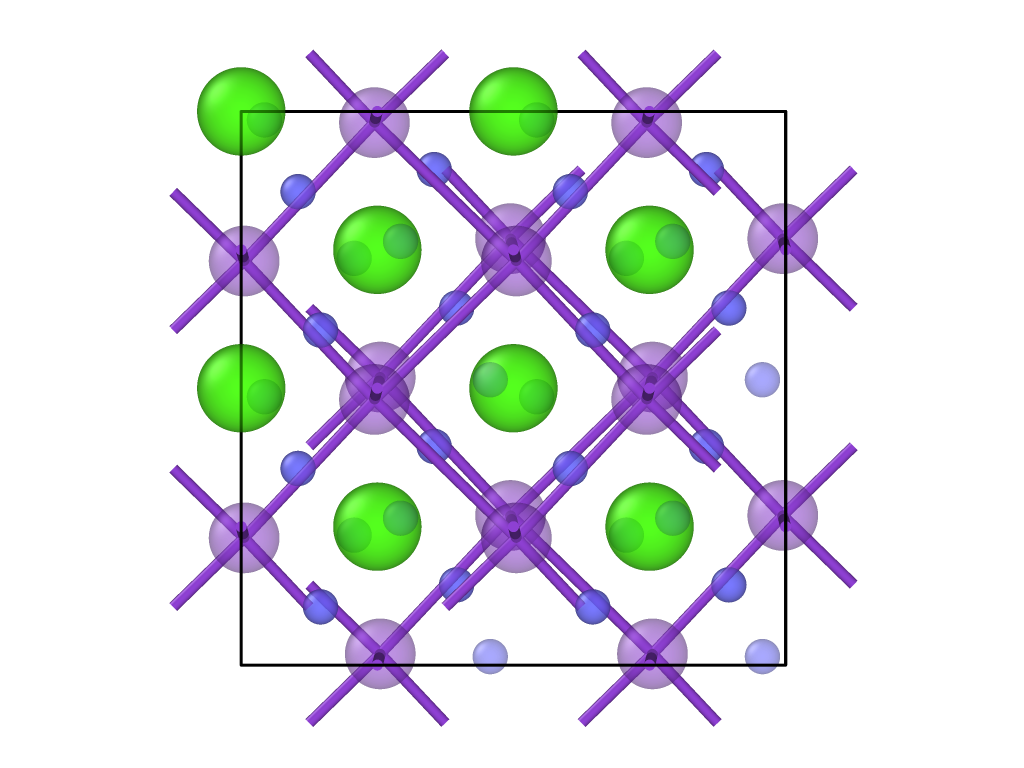
\includegraphics[width=.5\textwidth]{./data/plots/defects/062.05.KCaF3/plots/ref_front.png} \hfill
	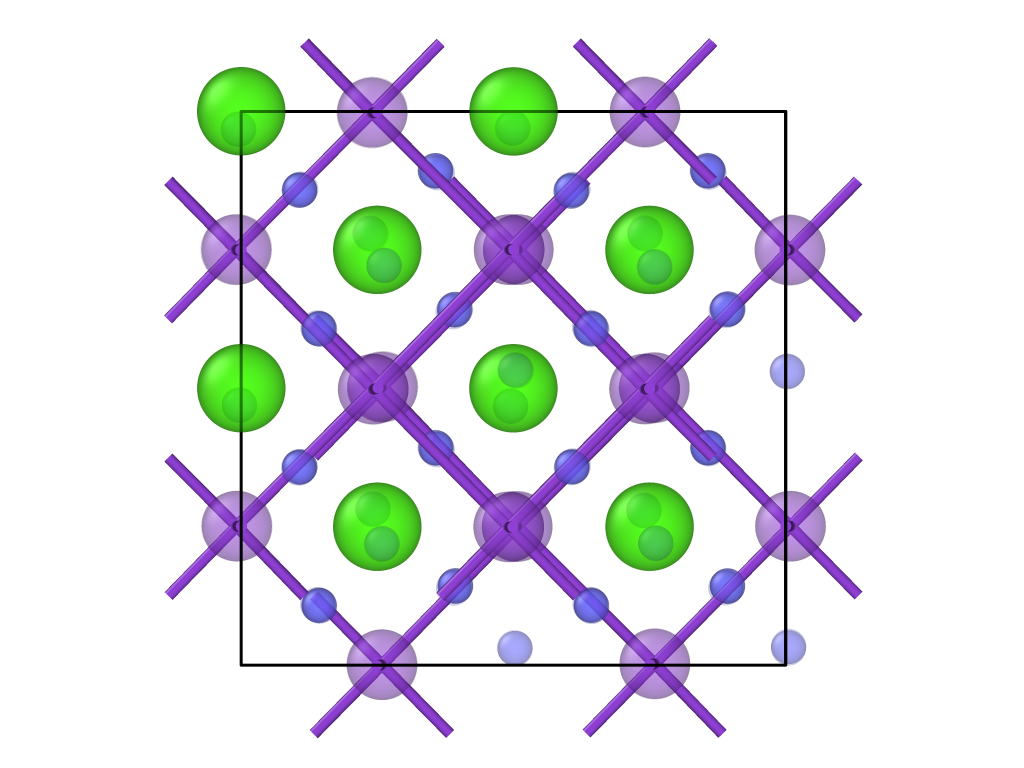
\includegraphics[width=.5\textwidth]{./data/plots/defects/062.05.KCaF3/plots/2_front.png} \\
	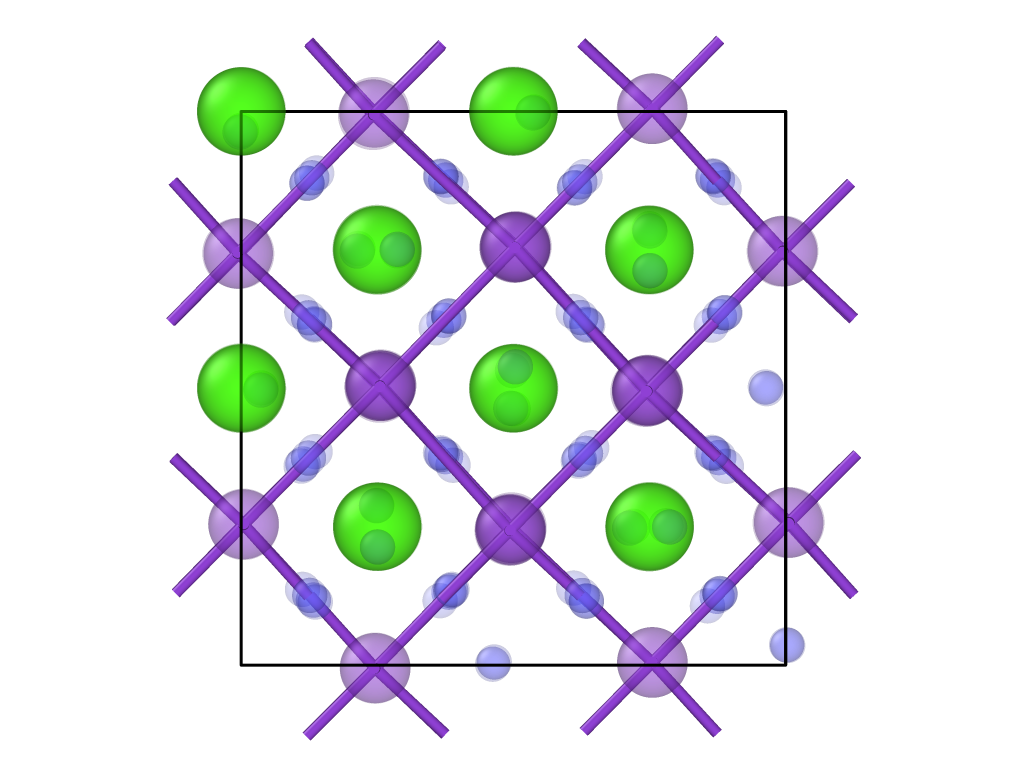
\includegraphics[width=.5\textwidth]{./data/plots/defects/062.05.KCaF3/plots/4_front.png} \hfill
	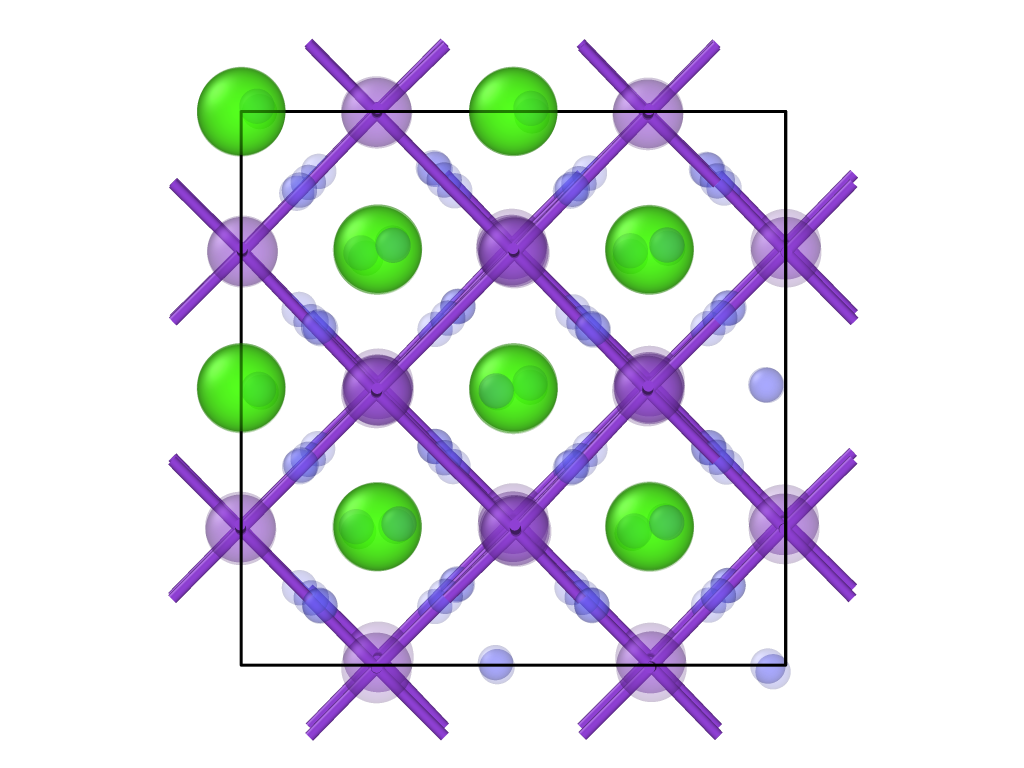
\includegraphics[width=.5\textwidth]{./data/plots/defects/062.05.KCaF3/plots/5_front.png}
	\caption{Front view along long axis.}
	\label{}
\end{figure*}

\begin{figure*}
	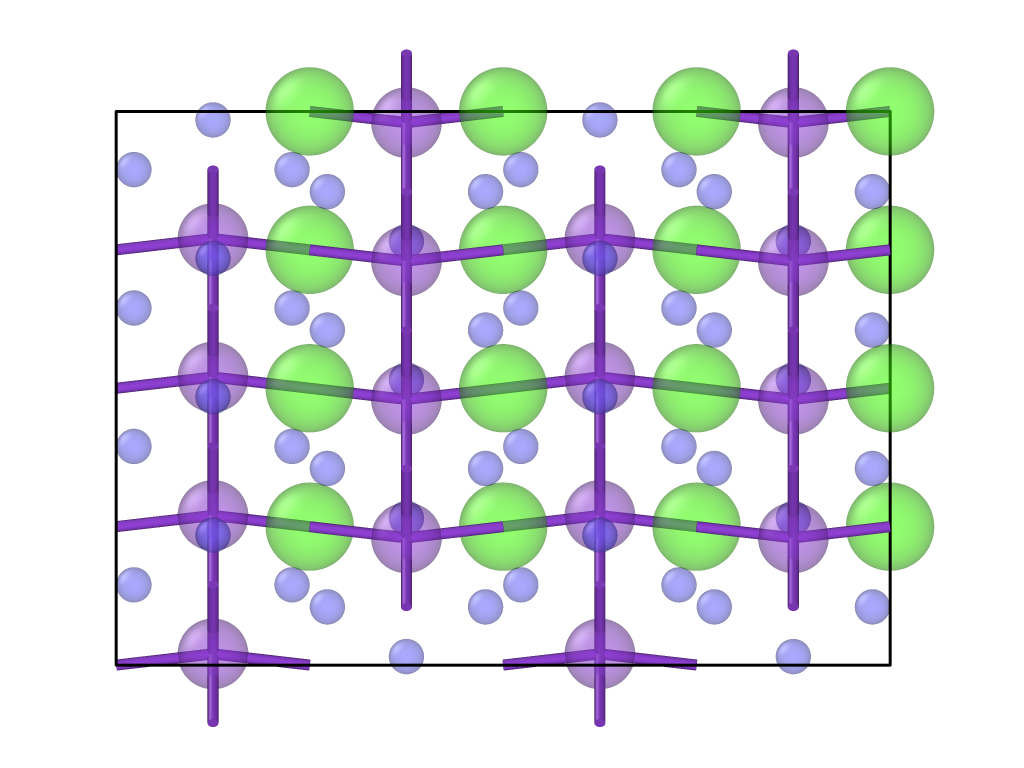
\includegraphics[width=.5\textwidth]{./data/plots/defects/062.05.KCaF3/plots/ref_left.png} \hfill
	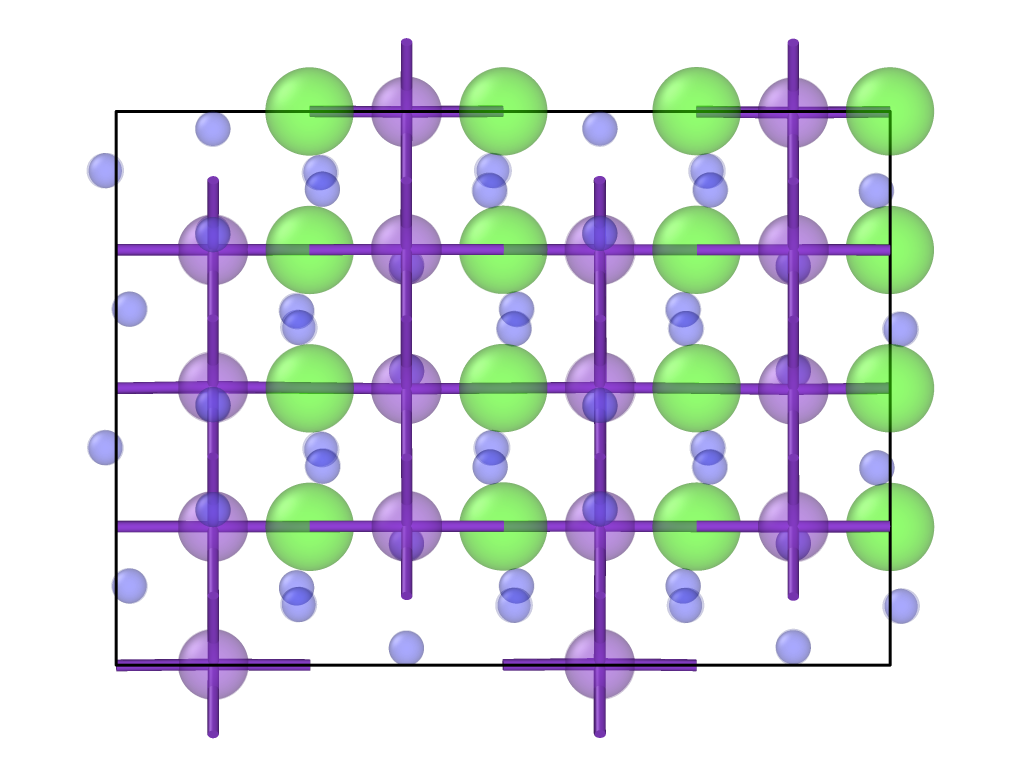
\includegraphics[width=.5\textwidth]{./data/plots/defects/062.05.KCaF3/plots/2_left.png} \\
	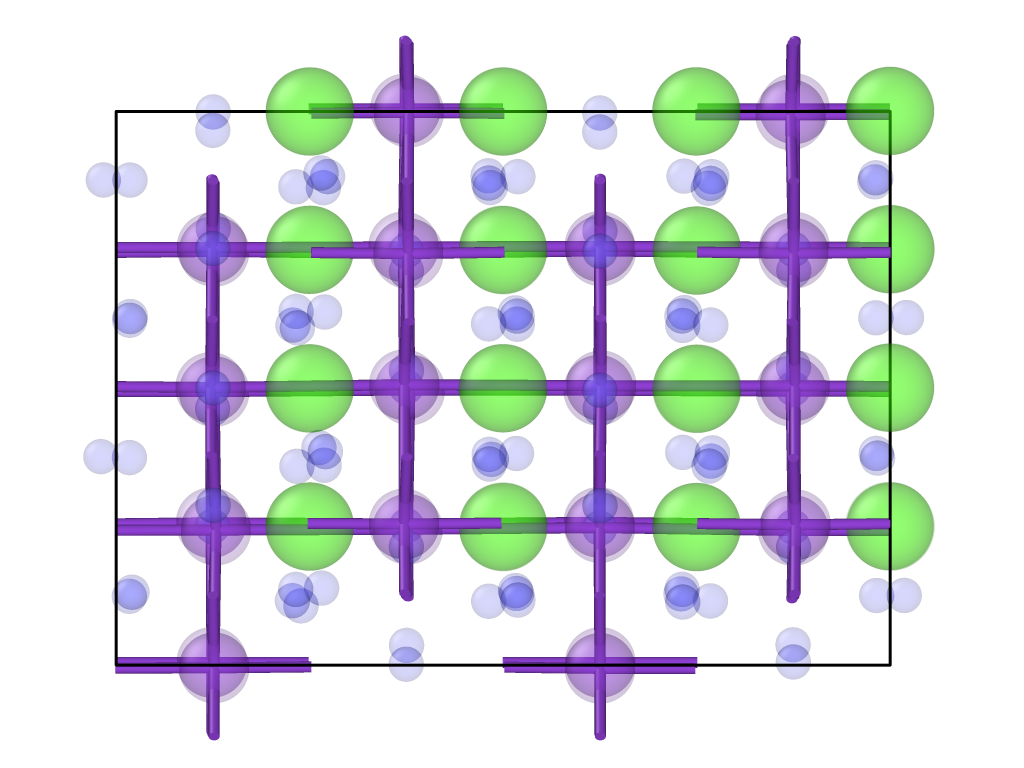
\includegraphics[width=.5\textwidth]{./data/plots/defects/062.05.KCaF3/plots/4_left.png} \hfill
	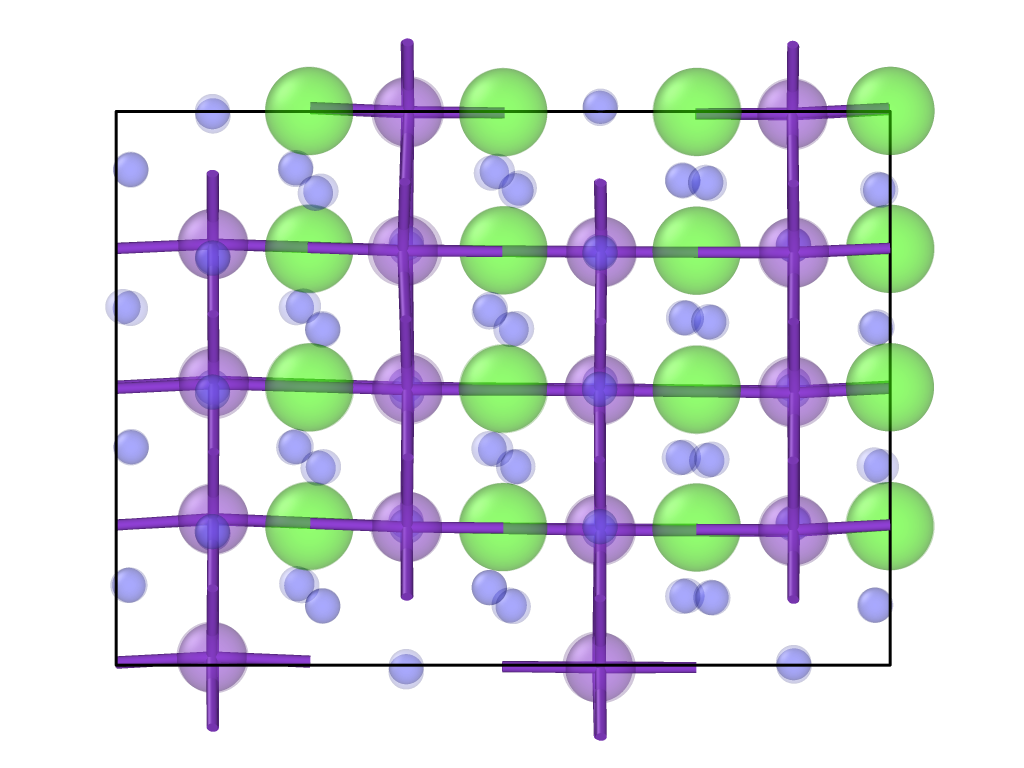
\includegraphics[width=.5\textwidth]{./data/plots/defects/062.05.KCaF3/plots/5_left.png}
	\caption{Left view along short axis.}
	\label{}
\end{figure*}

\begin{figure}
	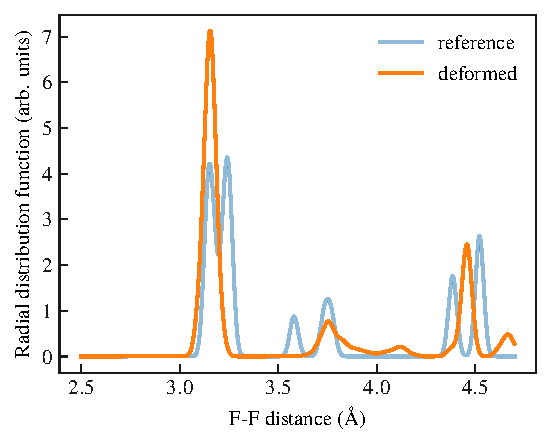
\includegraphics[width=\textwidth]{./data/plots/defects/062.05.KCaF3/rdf/geometry_in_def_4.pdf}
	\caption{RDF trajectory 4}
	\label{}
\end{figure}
